% !TeX root = ../main.tex
% Add the above to each chapter to make compiling the PDF easier in some editors.

\chapter{Approach}\label{chapter:Approach}
%In this chapter, the proposed solution to tackling pervasive computing and data distribution of context-aware input sensor data is unfolded. At the beginning, a broad perspective of the architecture is demonstrated, followed by, the explanation of modeling input sensor data. Then, two sections describing pervasive computing and data distribution models and architectures. Finally, a description of the communication model is disclosed.

\section{Requirements}
\section{Use Cases}
\section{Modeling of Input Sensor Data}
\subsection{Show how the different sensors have data been modeled to fit our requirements for further use in computations}



\section{Computation Model}
\newpage
\subsection{Dealing with Dependencies}
Before proceeding to examine the computation itself and explain how it is designed, we must first show what are the dependencies that the computation would need to execute. There are different types of dependencies; first are the software frameworks that the whole design relies on and must exist on each Node. These are the common libraries and systems that most of the computations would need to execute. That's why, these dependencies are shipped and configured in each Node in our design, examples of these dependencies include the operating system, data store, node-red and any other standard or custom libraries that is needed to guarantee a successful execution. In addition to, SCAMPI which must be included to allow communication between Nodes. These dependencies need only to be shipped once while initializing the Node.

 Second, are the dependencies that are specific to each computation such as additional scripts, data files or libraries. In this case, they cannot be shipped at Node initialization since we cannot know what are the custom dependencies any computation would need beforehand. Therefore, the design of the computation model allows a way to configure additional dependencies, which are sent accordingly to any Node that is going to execute this computation.
  This creates a bit of ambiguity because what if the dependency that is being shipped  already is on the receiving Node, also what makes it more complicated, is that the Node does not know if it is an older version of the dependency or a newer one. Furthermore, what if there is a computation on the Node that uses an older version of the same library while the maintainer is sending a new computation with a newer version of the same library that is not backward compatible. However, there are multiple proposed solutions to remove the ambiguity and make the custom dependency shipping more concrete; one solution would be to give the dependencies different names according to their versions before shipping them, hence, any different version would not replace the existing ones. Another solution would be to design a system that links each running computation on the Node to its dependencies and once a collision appears, the new computation renames its dependency and uses the renamed one.
 
\newpage
\subsection{Dealing with Resources}
Resources are a different type of dependencies which are also necessary for computations to run. However, they might differ or not exist at all on each Node, if one of the needed resources to carry out the computation is missing then it could be either dismissed or queued and that depends greatly on the type of resource. Moreover, the maintainers cannot make any assumptions about them, meaning, an assumption stating that each Node has a camera is not necessarily true. Since the resources cannot be standardized, each computation must specify the resources it is going to need, then a Node can check against its capabilities and decide whether it could carry out this computation or not. This kind of information is also known as computation meta-data. Resources may be classified into two main types explained below.

\subsubsection{Hardware Resources}

  Hardware resources  are attached to a Node such as cameras, temperature and gas sensors.  Also, executing a computation on a Node missing this type of resource should have a lower possibility of being queued, since its highly unlikely that this hardware resource would be attached soon. The computation model suggests several ways to describe a Node resource capabilities; first by using a specification file that expresses the resources in a certain Node. Of course this approach has its drawbacks since if we attach a new hardware resource we must also edit the specification file correspondingly and that increases the manual work. Secondly, by using operating system commands to discover the attached resources each time a computation needs to be deployed on a system. 
  
  Moving on to consider the risk of computations acquiring the same hardware resource at the same time, for instance, two computations that want to take a photo at the same time. This is problematic because whichever computation acquires the lock on the camera first will succeed while the other will fail. Therefore as a resolution, the design proposes resource decoupling; instead of having the computation ask a specific resource directly for information, the resource will always push its data to a database. Afterwards, the different computations could query the data from the database.
  

\subsubsection{Computational Resources }
The second type of resources is related to the Node performance, its power and memory capabilities. Computations vary in terms of resource consumption and hence a heavy computation should not be deployed to a Node which is already loaded. Considering that each computation model has meta-data describing its resource consumption, then it rather easy to decide if it is going to be deployed on a specific Node or not. Additionally, if it is not going to be deployed then it should be decided whether the computations is going to be queued or dismissed according to the possibility of acquiring the resource.




\newpage


\subsection{Execution Model}
- Which nodes should execute the data, is it all, some  or a specific nodes. Also, how is the model specified in the computation meta data.
- How do we know if a Computational Instance has been executed or not.

%\subsubsection{Computation Meta-Model}
Since the goal is to push computations to the available nodes which have the capability to do so, there are three main aspects that must be addressed to achieve this goal.
\begin{itemize}
	
	\item First, is to be able to express the computational requirements and resources that the computation is going to use while running on a specific node, which is also called \textbf{"Compuation Meta-data"}. Since we cannot make assumptions that a certain node has specific resources or specification as explained in \ref{subsub:node}, these requirements has to be pushed along with the computation. It includes, for instance, the amount of processing power and random access memory the computation is going to need, also, the resources required to perform such a computation.
	The meta-data is expressed as a \textit{JSON} formatted object.
	
	\textbf{include example}
	
	\item Second, is the core of the meta-model, which is a model expressing the computation itself, and since node-red is the chosen platform to execute our computation on, then naturally, it is modeled into a \textit{flow}, which is a model used by node-red to describe the capabilities and actions of a computation in JSON format. This simplifies the whole idea of making the computation meta-model travel through the network, because with node-red, the maintainer could develop a computation using the user interface of node-red, then export this computation as a flow, include the meta-data and publish it to the network. Afterwards, a node can read the meta-data and analyze if it could run this computation according to its resources, then import the flow into its node-red instance and deploy it for running.
	\textbf{include example}
	
	\item Last aspect in the meta-model is the output or results of the computation run. Since the node does not know what kind of data does the computation produce, therefore the maintainer must specify the way the output data is used or stored. In this case, nodes can understand whether the data needs to be sent back to the original node or just stored in a local database for further use. \\
	\textbf{include example}
\end{itemize}

\subsection{Input Output Modeling \& Flow Composability}
- Controlled vs Discovery (uncontrolled) nodes 
- Dealing with intermediate data
- I/O spec design for databases for two composable flows
- Compostability has the orthogonal issue of matching input/output "Controlled" IOSPec


\section{Moving Data}

\subsection{Data Streaming}
we can ask the hight performance units to stream from cameras no low devices. but how to do it ?

\subsection{Explain data distribution among several nodes to apply pervasive computing}

\subsubsection{Input Meta-data}
is it local, provided or collected data.
% moreover, the way that the input data used while doing this computation will be provided, whether it gets the input data from a local database or is it going to be included along with the computational data. 

\section{Networking}

\subsection{SCAMPI }

\section{System Design }
A System Design can be broadly described as an architecture of the system, which includes an explanation of each and every hardware component of the system, the connection between these components if there is any, and the data flowing between these components. Moreover, it provides a wide glimpse of the whole system but not its exact functionality, hence, giving a simple understanding of the architecture without jumping into much detail.\\
Initially, the components of the System Design is introduced, then, the connection between these components is shown, and eventually, the flow of the data is pointed out.

\subsection{Components}
\label{sub:components}
Below, each component of the proposed system design is explained.

\subsubsection{Node}
\label{subsub:node}
%The first set of components to explain are the sensors, they refer to objects that detect certain change in the environment and converts these changes into digital data and 
%which refer to objects that can detect certain changes in the environment and converts them to digital data, 
A Node is one of the core components of this design, it is a small computer device of low storage and computation capacity compared to nowadays portable computers, commonly a \textit{Raspberry Pi} but could be any other device. It is connected to several sensors which typically detect certain changes in the environment and converts it into digital data, for instance, Gas sensor, Temperature sensor or a Camera. Then, the device either stores the data into a local database, performs a computation locally, does both or even asks other nodes to do computation instead, however, an assumption about which sensors or specifications does a specific node  possess can not be made, meaning, each node might not have the exact number or types of sensors because each node may be deployed in a different timing or context. Thus, each node has a configuration file specifying its capabilities. A typical node is shown in figure \ref{fig:node}

\begin{figure}[H]
\centering
 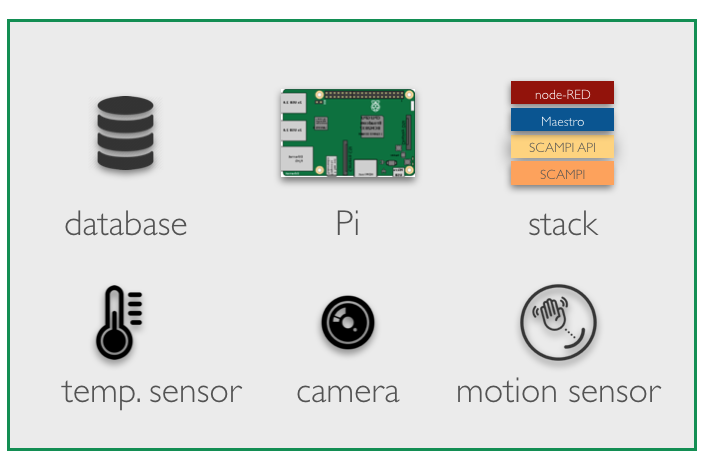
\includegraphics[scale=0.4]{images/node.png}
 \caption{A typical node in the system}
 \label{fig:node}
\end{figure}

\subsubsection{High PerformanceGraphics Processing Units }

A High Performance UnitGraphics Processing Unit \textit{GPU} is a device with massively parallel architecture designed to handle multiple tasks at the same time, thus observed to be much faster and more efficient than a Central Processing Unit \textit{CPU}, and in turn, has higher computation capabilities than the CPUs in the proposed system nodes in \ref{subsub:node}. An example of a high processing unit is  a Graphics Processing unit \textit{GPU}.

\begin{figure}[H]
	\centering
	
\includegraphics[scale=0.7]{images/gpu.png}
		\caption{Figure denoting a Graphics Processing Unit GPU}
	\label{fig:gpu}
\end{figure}

\subsubsection{Network}
\label{subsub:network}
A Network in this design is a set of connected components which are capable of communicating and therefore allowing data sharing between them.
\begin{figure}[H]
	\centering
	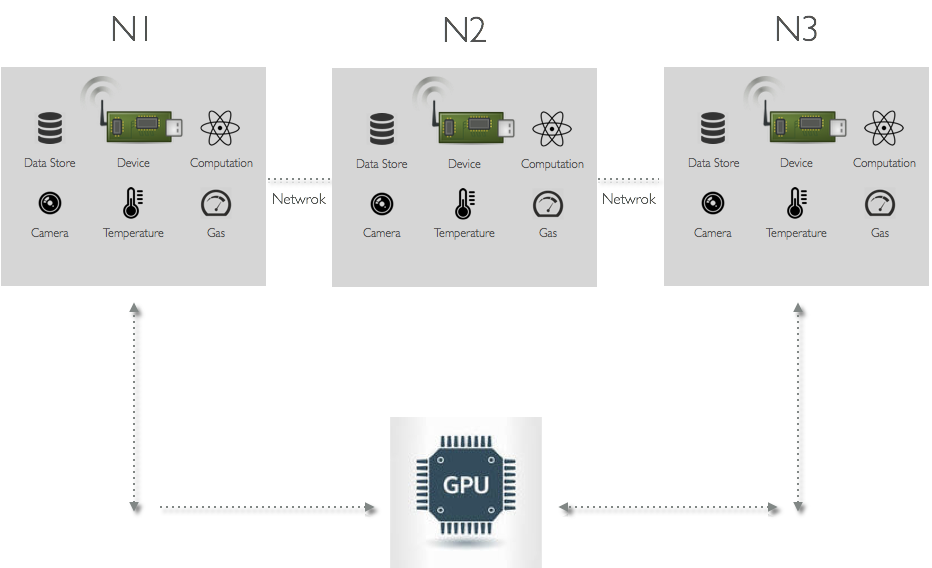
\includegraphics[scale=0.4]{images/network.png}
	\caption{A network consisting of three connected nodes and a GPU}
	\label{fig:network}
\end{figure}
-- TODO: 
Emphasis the difference between persistent and non persistent network links in system design.

\subsubsection{Mobile Device}
A Mobile Device in this context is any device that can connect to the network containing the nodes and is allowed to  carry data from one network to another, hence, allowing a form of data sharing between networks or nodes which are not connected.

\begin{figure}[H]
	\centering
	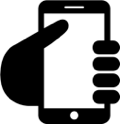
\includegraphics[scale=0.3]{images/mobile.png}
	\caption{Figure denoting a Mobile Device}
	\label{fig:mobile}
\end{figure}



\subsection{Connectivity and Data Flow}
A Network described in \ref{subsub:network}, is a simple form of connectivity between components, however, components and specifically nodes are not necessarily connected, sometimes they are just a standalone component that cannot share any information via direct connectivity, also, networks could be disconnected as well, meaning, a network might not be connected to the whole system, thus, is a standalone network. In these cases, a mobile device could help in carrying information and data between these disconnected nodes or networks. 

\begin{figure}[H]
	\centering
	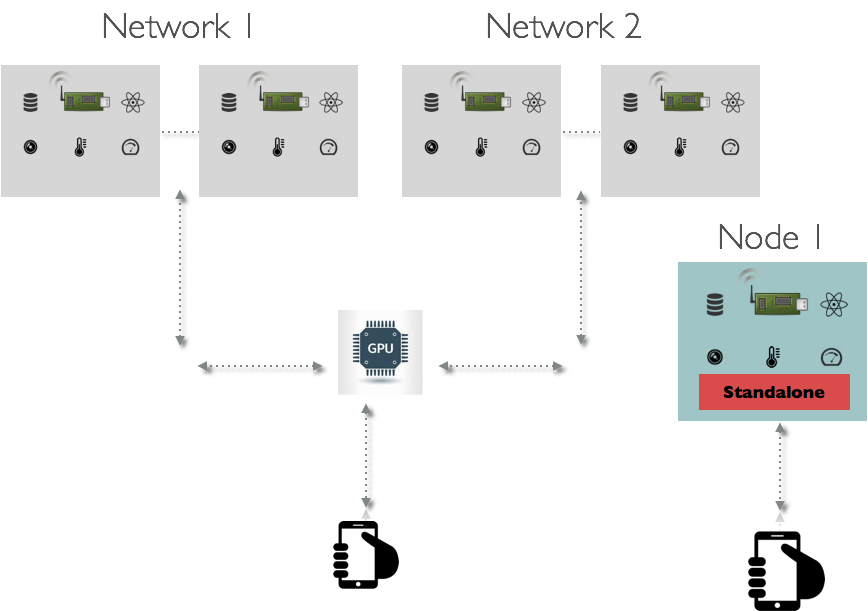
\includegraphics[scale=0.5]{images/system.png}
	\label{fig:system}
	\caption{Two networks connected with a GPU and one standalone network}
\end{figure}









\section{Summary}



